% !Mode:: "TeX:UTF-8"
\documentclass[10pt,a4paper,notitlepage]{report}
\usepackage{ifxetex,ifluatex}

\newif\ifxetexorluatex
\ifxetex
  \xetexorluatextrue
\else
  \ifluatex
    \xetexorluatextrue
  \else
    \xetexorluatexfalse
  \fi
\fi

% Better rendition of computer modern.
\usepackage{lmodern}

\ifxetexorluatex
    \usepackage{fontspec}
\else
    \usepackage[utf8]{inputenc}
\fi

% For mathematical typesetting.
\usepackage{amsfonts,amsmath,amsfonts,amssymb}

% For formal grammar.
\usepackage{syntax}

% For typeset diagrams
\usepackage{bytefield}
\usepackage{dirtree}

% Provides an extended tabular environment.
\usepackage{tabularx}

% For images.
\usepackage{graphicx}
\usepackage{float}

% For better enumerations.
\usepackage{enumitem}

% For source code listings.
\usepackage{listings}

% For fancy captions.
\usepackage{caption}

% For hyperlinks and fancy citations.
\usepackage[colorlinks=true,linkcolor=black,citecolor=blue,urlcolor=blue]{hyperref}

% Setting page geometry.
\usepackage[left=4cm,right=2cm,top=2cm,bottom=2cm]{geometry}

% Sets spacing between paragraphs
\setlength{\parskip}{0.8em}

% Default caption form
\captionsetup{labelfont=bf,textfont=it,justification=centering,font=footnotesize}

% Shamelessly pinched from 'dbaupp'. cheers!
% http://tex.stackexchange.com/questions/51645/x86-64-assembler-language-dialect-for-the-listings-package
\lstdefinelanguage
    [x64]{Assembler}     % add a "x64" dialect of Assembler
    [x86masm]{Assembler} % based on the "x86masm" dialect
    {   % with these extra keywords:
        morekeywords={
            CDQE,CQO,CMPSQ,CMPXCHG16B,JRCXZ,LODSQ,MOVSXD,
            POPFQ,PUSHFQ,SCASQ,STOSQ,IRETQ,RDTSCP,SWAPGS,
            SYSCALL,
            rax,rdx,rcx,rbx,rsi,rdi,rsp,rbp,
            r8,r8d,r8w,r8b,r9,r9d,r9w,r9b
        }
    }

% Alias python [2] to python. Add missing yield
\lstdefinelanguage
    [2]{Python}
    []{Python}
    {
        morekeywords={yield}
    }

% Remove the print and exec statements from python to make python [3].
\lstdefinelanguage
    [3]{Python}
    []{Python}
    {
        morekeywords={yield},
        deletekeywords={print,exec}
    }

% Straight quotes, please.
%\lstset{upquote=true}
\lstset{basicstyle=\ttfamily}

\author{Elliot Thomas\\ \small Supervisor: Sean Tohill\\ \\ University of Westminster}
\title{Network Packet Capture Generation and Falsification}
\date{\today}

\begin{document}
\maketitle
\begin{abstract}
\begin{center}
A document describing the design and development of a tool to assist in the crafting of network packet captures for educational purposes.
\end{center}
\end{abstract}
\pagebreak
\listoffigures
\lstlistoflistings
\tableofcontents

%%%%%%%%%%%%%%%%
% Introduction %
%%%%%%%%%%%%%%%%
\chapter{Introduction}
Education is important. Education is one of the underpinnings of a progressive society, along with law and order and a few other things.
Despite this, it seems human ingenuity is education's greatest enemy. Humans are lazy - most of us will strive to do as little work as possible for the greatest gain.
We seek to make our lives better, easier, all to spend more time on the things we enjoy. For many, this will be leisure activities, for some, socialising, the humble few may take joy in altruism.

But motivations are irrelevant here, just the effects.
In academia, plagiarism is a problem - people are unwilling to put the time in to do their own work. They realise that if someone else has solved a problem identical to theirs, they could just reuse that.
What these people fail to realise, is that there is no substitute for experience. This problem is relevant in all fields, academic or applied, practical or theoretical; computer security and forensics is no exception.

\section{Reader level}
The reader is expected to be somewhat familiar with networking terminology and forensic analysis techniques. Basic knowledge of Python will be required to understand the design and implementation chapters.

\section{The problem}
Teaching network security and forensics is aided greatly by the presentation of example packet captures. These are used to learn and practice analytical skills, and to assess the level of understanding and knowledge that students hold.
Creating such packet captures is not difficult, but there are few, if any tools available for automating the process. Changing this is the purpose of this project.

\pagebreak

\section{Existing Solutions}
\label{sec:existing}
None, it would seem.

There are a number of tools for network packet capture, and a number of tools for analysing them. These tools do not solve the problem \emph{per se}, but do allow packet capture manipulation to a certain extent, and therefore might be a useful aid in manipulating packet captures.

\subsection{editcap}
Editcap is a program distributed as part of Wireshark.\\
From the manpage\cite{editcap-man}:
\begin{quote}
\textbf{Editcap} is a program that reads some or all of the captured packets from the \underline{infile}, optionally converts them in various ways and writes the resulting packets to the capture \underline{outfile} (or outfiles).
\end{quote}

For the purposes of assisting generation, this program allows splitting a file into a series of files, according to the time they were sent; i.e., splitting every 2 seconds (where each set represents a packet capture and each number represents the time a packet arrived):\\
\indent (1, 1, 2, 3, 5, 7, 8) $\rightarrow$ (1, 1, 2), (3), (5), (7, 8)

\subsection{tshark}
Tshark is a program distributed as part of Wireshark.\\
From the manpage\cite{tshark-man}:
\begin{quote}
\textbf{TShark} is a network protocol analyzer. It lets you capture packet data from a live network, or read packets from a previously saved capture file, either printing a decoded form of those packets to the standard output or writing the packets to a file.  \textbf{TShark}'s native capture file format is \textbf{pcap} format, which is also the format used by \textbf{tcpdump} and various other tools.
\end{quote}

As stated, it acts as a network traffic capture and analysis tool. It has functionality that will identify packets by protocol (and can reconstruct TCP streams) and allows the user to filter them. This is useful functionality, as it allows you to remove packets based on the protocols they contain, making captures simpler to understand.

\subsection{Bit-Twist}
Bit-Twist is a tool suite containing a packet capture 'generator' (a traffic replay program, not unlike tcpreplay\cite{tcpreplay-web}) and a pcap editor.
From the website\cite{bittwist-web}:

\begin{quote}
With Bit-Twist, you can now regenerate your captured traffic onto a live network! Packets are generated from tcpdump trace file (.pcap file). Bit-Twist also comes with a comprehensive trace file editor to allow you to change the contents of a trace file.
\end{quote}

This tool is \emph{very} close to the desired utility. It permits editing a packet capture in a handful of ways, specifically:
\begin{itemize}
\item Appending a `payload' (arbitrary bytes) to the end of every packet.
\item Removing a range of bytes from every packet.
\item Recalculating checksums for (non-fragmented) IP, TCP, UDP and ICMP packets.
\item Saving a specific range of packets either by their occurence (i.e. The fourth packet to the seventh packet) or by their timeframe (i.e. all packets between 2006/10/1 00:00:00 and 2006/10/31 10:30:00).
\item Truncating packets to a specific 'layer' - where 2 is the link layer, 3 is the network layer and 4 is the application layer.
\item Restricting edits to a specific 'header'- Ethernet, ARP, IP, ICMP, TCP and UDP are supported in this case.
\end{itemize}

\section{Conclusions}
There are tools that can help, but nothing particularly geared towards the problem. Most existing tools present a kind of `read-only' interface toward existing captures, or allow modifying them while preserving packet integrity. Bit-Twist's pcap editor allows arbitrary modification, but is somewhat cumbersome to use, applying the same changes on all packets.

%%%%%%%%%%%%
% Research %
%%%%%%%%%%%%
\chapter{Research}
\section{Approaches to the Problem}
The problem `\emph{How does one generate unique packet captures for teaching analysis to students?}' is open to multiple solutions. In this project, three possible approaches were considered. These can be described as \emph{synthesis}, \emph{generation} and \emph{composition}.

\subsection{Synthesis}
This would work as a program that understands a \emph{scenario} defined in a kind of declarative language, that creates a set of unique permutations of that scenario by varying some key data (names, hosts, times etc.) and the exact sequence of events. From this, it would synthesise a complete packet capture from each scenario - carefully constructing every packet - such that all generated captures represent the same abstract event (i.e. corporate espionage) but with wildly different specifics, hindering collusion.

This approach has the advantage of a flexible interface and fast implementation - at the cost of having to understand and reproduce the complexity of various networking protocols and producing a completely artificial output.

\subsection{Generation}
Much like \emph{synthesis}, this would understand a declarative language for describing a scenario, but this approach would be to program a network of computers to actually do the actions in the scenario rather then synthesise their side effects. This would then run a packet sniffer on this network, generating perfectly authentic network captures of a real network, but where the human actors in a scenario are emulated by computers.

This approach has the advantage of flexibility and authenticity - at the cost of being very inefficient and fragile. It is more then likely such an approach would use a network of virtual machines running real-world operating systems and protocol implementations. This introduces a fair amount of unpredictability (which is both a good and bad thing), and would require changes if/when a used interface changes.

\subsection{Composition}
This was the first approach considered, and is perhaps the simplest. This would be a program that takes a set of existing packet captures (ideally, small purpose-built captures representing single transactions) and combines them while altering things like hosts, times and the like.

This approach has the advantage that real-world scenarios can be used - an existing library of captures will still be useful to provide a data source for the program - and it retains a degree of authenticity. It has a lesser variant of the downside that \emph{synthesis} has, in that it will need to identify and modify various networking protocols, but does not need to understand how they work - which removes a great deal of complexity. It also depends on existing captures - if these aren't available, the tool cannot function.

\subsection{Chosen Approach}
\emph{Synthesis} and \emph{generation} approaches are very complex - a good implementation would take a considerable amount of time to write and test, and allow a lesser degree of control to the user. For this reason, a \emph{composition} based approach was chosen - it is comparatively simple and easy to understand; desirable qualities for any tool.

% Programming language criteria
\section{Programming language: Criteria}
Choosing a programming language is, obviously, a decision that needs to be made, and there is no single correct choice. There are many factors influencing such a decision, each one needs to be considered. There were three major factors considered in this decision:
\begin{enumerate}[label=\roman*)]
\item Requirements - what does the program require?
\item Knowledge - how difficult will it be to program in and maintain?
\item Availability - on what platforms can projects using this language be used?
\end{enumerate}

\subsection{Requirements influence}
At its heart, this project is a data processing project. There are no requirements for real-time processing, no requirements for concurrency, no requirement to make use of or implement a specific API nor requirements for any kind of interactive behaviour. This project can very easily be designed and implemented as a batch program - give input, run program, get output.

Given the minimalistic requirements of the program, just about any Turing-complete language is serviceable. As such, the decision will have to be made predominantly on the other three factors. That's not to say entirely, some languages lend themselves quite well to generic data manipulation, while others are more specialised and geared towards specific purposes. For instance, Javascript is more suited towards web-based projects (given that its usual interpreter is a web browser), while C, Java and Python are more general purpose. Haskell, Java and Python have good support for abstract data structures while various assembly languages barely have the notion of a data type.

One important factor is for the program to be easily extended. While it is possible to write an extendible program in just about any language, it helps considerably if there is support for loading code from an external source at runtime, i.e. to allow building a plugin architecture.
Most languages or platforms allow this in some manner (and practically all platforms depend on doing this in one way or another - this is how shared libraries work). While POSIX platforms provide functions like \lstinline$void *dlopen(const char *filename, int flag);$, this interface is not consistently available on non-POSIX platforms, and requires code to be compiled first. Meanwhile, Python, Javascript and even Bash provide methods for loading new code programatically without the need to compile code first, allowing for a very flexible, powerful and user-friendly system to be developed.

\subsection{Knowledge influence}
Knowledge is a subjective factor that pertains to the programmer(s) developing the project. It is a limiting factor; a programmer proficient in C is not necessarily going to be able to understand a very different language such as Haskell. Also worth mentioning is simple preference - while not a overriding factor - can help shape a choice.

\subsection{Availability influence}
Availability for most languages is somewhat of a non-issue. Given that portability is a desirable outcome, only languages which have a usable and consistent enough implementation across platforms will be considered. This eliminates some languages such as C\#, Visual Basic (or any .NET language).

It is also worth noting portability - are there provisions for file input/output? In the case of the various assembly languages, this is left to the programmer. Even if the assembly language itself is abstract and portable, it only dictates how the processor is used - assembly often leads to some \emph{very} specific code.

\begin{lstlisting}[
	language={[x64]Assembler},captionpos=b,
	caption={[64-bit assembly example]Written for x86-64 processors, this uses Linux's 64-bit system call convention to write data to 'stdout' (standard output)}
	]
mov rax, 1   ; system call constant for write on Linux64
mov rdi, 1   ; first argument: file descriptor to write to, eg: stdout.
mov rsi, msg ; second argument: buffer holding data to be written.
mov rdx, len ; third argument: number of bytes to write.
syscall      ; Do the system call. Similair to int 0x80.
\end{lstlisting}

\section{Programming Language: Assessment}
Many languages were assessed for use in this project using the criteria above, with some being discarded on a singular fatal flaw. These are:
\begin{itemize}
\item C\#, Visual Basic, other .NET languages: These are fairly portable with the advent of Mono\cite{mono}, but the author still has reservations about this.
\item Haskell: An interesting language, but requires a substantially different approach to program design than the author is familiar with.
\item PHP, Javascript: Languages that are perfectly serviceable for the task at hand, but have a heavy focus on web development rather then packet capture processing. A more neutral choice would be better.
\item Assembly: These languages are very low level and require a great deal of effort to accomplish simple tasks. Additionally, they tend not to be portable.
\item COBOL: An affront to language design, this is on the list purely as humour.
\end{itemize}

\subsection{C}
For a while, C was the \emph{lingua franca} of the programming world. C is a fairly old language, dating back to 1972 and was used to write many parts of the UNIX operating system\cite{tcpl}.

C is technically considered a high-level programming language, in that it gives you automatic variable allocation and permits arbitrarily complex arithmetic and logical expressions without explicitly storing intermediary results. The detail of a register (memory that is part of the CPU) is seldom expressed in C code; variables have an addressable place in main memory unless the register keyword is used in variable declaration\footnote{Although, an optimising compiler \emph{can} do this for you.}.

C has the advantage of very little overhead - there is no garbage collector; all memory management is done manually. Given that networking protocols, particularly the ones relevant to this project, are often implemented in C; C seems like a fair choice despite its shortcomings.

Perhaps the biggest issue with using C is work to functionality ratio. Data structures available in other languages like linked lists and hash tables require implementing, and code generally has to be quite explicit. There are no abstractions such as `iterate over every element in this array' provided by default (although this is possible to some extent with preprocessor macros), and C is not an object oriented language - there is no real notion of classes, which are (if used correctly) a useful abstraction.

C is a compiled language, which means the project requires compilation to a platform specific executable. While the code in itself is no less portable for this, it does require testing on compliers for all supported platforms - most of which are not completely compatible with each other.

\subsubsection{C++}
Often described as `C with classes', C++ is a derivative (for the most part, a superset) of the C programming language\cite{tcpppl}.
C++ adds classes, namespaces, `references' and templates to the C language. For the most part, it retains compatibility with the C language and can be freely mixed with C code.

C++ resolves some of the issues with using C for this project. However, the remaining issues make C/C++ difficult to choose.

\subsection{Java}
Java is a language usually compiled to \emph{bytecode} and then interpreted by a virtual machine, the Java Virtual Machine (JVM). The virtual machine accepts programs in a standardised form, so Java bytecode can work on multiple implementations. This means that Java programs, once compiled, can be run anywhere\footnote{It should be noted that other compilers exist - GCJ\cite{gcj} is such an example that compiles Java into machine code.}. Java is a very popular language\cite{javatech}, used in enterprise environments and commonly taught to university students doing a course in computer science.

Java is a strongly typed, partially object oriented language - it supports all typical object oriented abstractions, but also supports \emph{primitive types} and treats classes and methods differently to other objects (you cannot assign them like other objects).

Java has the advantage of executable portability that C and C++ do not, and is almost perfect for this task. It supports loading bytecode at runtime and has support for file I/O.

The only real issue is somewhat subjective - the author finds Java code needlessly verbose. This is discussed in the verbosity section (\ref{sec:verbosity}).

\subsection{Python}
Python is an interpreted, multi-paradigm, fully object oriented language. Python also has its own philosophy - solutions are often deemed to be \emph{pythonic} based on various factors such as elegance and being obvious. However, in Python, mechanism is separate from policy; the various Python conventions are exactly that - conventions.

Python code is usually distributed in source form, but can be compiled to a bytecode not unlike Java. Python as a language does not enforce any kind of information hiding or encapsulation, and does \emph{not} require nor support typed variables\footnote{Note that this does not mean python is weakly typed -  Python has strong typing that requires explicit conversion.}. This is in contrast to Java, which provides these kind of access qualifiers. Instead of these, a convention is used - private and protected access qualifiers are signified by a single underscore before member names, and API documentation is generally used to specify argument and return types for functions and methods.

\subsection{Code Verbosity}
\label{sec:verbosity}
Code verbosity is a problem in certain languages, and can make even simple code hard to follow - the less you have to read, the quicker you can comprehend it.
\pagebreak
To illustrate this problem, consider a simple task: write a program that counts the number of lines in a text file.
In the interest of fairness, the program will have specific behaviour; it should accept standard input or a file path as its first command line parameter, and work by looking at each character in the file and comparing it to a line feed. If reading from a file that does not exist, it should print an error message. Additionally, all variable identifiers should be the same or similar when translated to code.\footnote{The author recognises that code style has an impact on the metrics used (line count and source file size), and that all of these programs can be rewritten to occuply less space, however doing so would render them neigh-unmaintainable.} 

This program was fully implemented for the three considered languages - C, Java and Python. The C implementation is as follows:
\lstinputlisting[
	language={C},label={lst:nol.c},numbers=left,
	caption={Number of Lines program, in C}
]{nol.c}

The C version's program source code consists of 38 lines and occupies 514 bytes of storage. This version of the program produces the correct output of 38 when run on its own code, 50 and 22 when run on the other two versions' code.
\pagebreak

The Java version, with full exception handling as requested by the Java compiler, looks like this:
\lstinputlisting[
	language={Java},label={lst:nol.java},numbers=left,
	caption={Number of Lines program, in Java}
]{nol.java}

The Java version is considerably larger, consisting of 50 lines and is 1113 bytes large. This version also produces correct behaviour.
\pagebreak

The Python version, in Python 3, looks like this:
\lstinputlisting[
	language={[3]Python},label={lst:nol.py},numbers=left,
	caption={Number of Lines program, in Python}
]{nol.py}

The python version is the smallest, at just 22 lines and 371 bytes in size. Again, correct behaviour is observed.

\subsection{Chosen Language: Python}
Time was the unspoken major factor in this decision, and given the liberty to choose any programming language means ones in which the programmer has experience will take precedence. This means that languages designed for unfamiliar paradigms (such as Haskell, being a purely functional programming language\cite{haskfunc}) or languages that leave a considerable amount of work to their user (such as Assembly) were eliminated.

The choice was Python. This was driven by its status as a multi-paradigm language that offers different models of program abstraction.
To illustrate this, shown below are two functionally equivalent and compatible prime number \emph{iterators};
\begin{lstlisting}[
	language={[3]Python},label={lst:ooprime},
	caption={[Python primegen, object style]An object oriented approach to a prime generator.}
]
class primegen:
    def __init__(self, start, end):
        self.cur = start
        self.lim = end

    def __iter__(self):
        return self

    def __next__(self):
        prime = False
        while not prime:
            if self.cur >= self.lim:
                raise StopIteration()
            for i in range(2, self.cur/2):
                if self.cur % i == 0:
                    break
            else:
                retval = self.cur
                prime = True
            self.cur += 1
        return retval
\end{lstlisting}

\begin{lstlisting}[
	language={[3]Python},label={lst:ooimp},
	caption={[Python primegen, imperative style]An imperative approach to a prime generator.}
]
def primegen(cur, lim):
    while cur < lim:
        for i in range(2, cur/2):
            if cur % i == 0:
                break
        else:
            yield cur
        cur += 1

\end{lstlisting}

\subsection{Python 2 or Python 3?}
Like most languages, Python has versions. The Python language currently exists as two distinct versions, Python 2 and Python 3. This is not to be confused with the multiple implementations of Python - which can support the same language and standard library - but the actual grammar of the language.

\subsubsection{What is wrong with Python 2?}
As a language, Python 2 made some odd decisions. Firstly, it had a `print' statement - which sounds perfectly reasonable until you need to accommodate for edge cases and specific behaviour. Print statements have the form;
\begin{grammar}
<expressions> ::= <expression> | <expression> `,' <expressions>

<print statement> ::= `print' <expressions>
\alt `print' <expressions> `,'
\end{grammar}

which means that
\begin{lstlisting}[language={[2]Python}]
print "a", "b", "c"
\end{lstlisting}

is distinct from
\begin{lstlisting}[language={[2]Python}]
print "a", "b", "c",
\end{lstlisting}

The former outputting ``a b c'' followed by a newline, and the latter outputting ``a b c'' without a newline! There is no convenient way of changing what the item separator is, requiring setting a field in the `sys' module. The exec statement has similar issues.

Furthermore, Python 2 has some odd semantics for its `input' function, which will read a line of standard input, and then \emph{evaluate this input as a Python expression}. In order to read the unevaluated input, `raw_input' is needed.

Python 2 evolved in such a way to have two different object orientation systems. Python 2 has \emph{old-style} classes and \emph{new-style} classes, observe:

\begin{lstlisting}[language={[2]Python}]
>>> class Foo:
...  pass
... 
>>> class Bar:
...  pass
... 
>>> class Quux(object):
...  pass
... 
>>> f = Foo()
>>> b = Bar()
>>> q = Quux()
\end{lstlisting}

Here, two (empty) \emph{old-style} classes `Foo' and `Bar' are defined, along with a \emph{new-style} class `Quux'. Instantiation is identical for all of them, however...

\begin{lstlisting}[language={[2]Python}]
>>> type(f)
<type 'instance'>
>>> type(b)
<type 'instance'>
>>> type(q)
<class '__main__.Quux'>
\end{lstlisting}

Their \emph{type} differs. All \emph{old-style} objects have a type of `instance' while \emph{new-style} objects have a type matching their class.

\begin{lstlisting}[language={[2]Python}]
>>> type(f) == type(b)
True
>>> type(f) == type(q)
False
\end{lstlisting}

Python 2 also shares a limitation common to early, ``lower level'' programming languages like C in that it does not distinguish between a \emph{string of characters} and a \emph{string of bytes}.
This makes handing either somewhat cumbersome. For instance,

\begin{lstlisting}[
    language={[2]Python},
    caption={[Python 2 character length] The pound sign, with a length of two characters.}
]
>>> len("£")
2
\end{lstlisting}

Which makes sense only when considered as a UTF-8 encoded characer, which exists as $(194, 163)$ representing codepoint $163$ in unicode.
Python 3 provides a better abstraction - strings are arrays of characters, `bytes' are arrays of integers in the range $0 \rightarrow 255$, and strings can be encoded to bytes using a variety of different encodings.

\begin{lstlisting}[
    language={[3]Python},
    caption={[Python 3 character length] The pound sign, with a length of one character.}
]
>>> len("£")
1
\end{lstlisting}

This is a rather important and useful distinction when dealing with predominantly binary data such as captured packets.

Perhaps the most compelling reason is that the reference implementation, CPython, currently exists as CPython 2.7 and CPython 3.4, with 2.7 being in maintenance mode\cite{cpy2maint} - that is, bug fixes only.

\section{Architecture}
There are many different ways of categorising programs, but most programs have a important, distinctive piece of behaviour that can place a program in one of two mutually exclusive categories. That is, are they \emph{interactive} or not.

In the context of program design, an interactive program is one that accepts and alters its behaviour based on human input.
A prime example of an interactive program is a text editor - it accepts input in the form of a series of keyboard presses and interprets each of these as a command to write a corresponding character.

Conversely, a non-interactive program is one that does \emph{not} accept user input. For instance, a compiler is generally non-interactive - it takes input in the form of source code, and produces output in the form of compiled code.

The author, being a Linux aficionado, is particularly fond of following the \emph{UNIX philosophy} where appropriate. This philosophy has no formal definition, but was once summarised, in the words of Peter H. Salus\cite{qcou},
\begin{quote}
This is the Unix philosophy: Write programs that do one thing and do it well. Write programs to work together. Write programs to handle text streams, because that is a universal interface.
\end{quote}

To this end, a system based around multiple small utilities that can be strung together to produce the desired output seems an appropriate architecture. Out of necessity, \emph{text} will not be used as a model for data, but a ubiquitous packet capture format will be used. It is evident from the programs listed in section \ref{sec:existing} that this format is \emph{pcap}.

\section{Development Methodology}
The widely known `waterfall model' of software development was, in its current form, presented as a flawed model that lacked development stage feedback\cite{wwr-waterfall-notes}. The waterfall model is fairly simple, it suggests a requirements analysis stage, followed by a linear progression of design, implementation, testing and finally maintenance. It works in an idealised scenario where all requirements are specific, well understood and concrete, and that there are no unforeseen problems in implementation. Unfortunately, this is not how things work in practice.

As the project will consist of lots of small components, with a tree-like dependency graph, it is possible to design, build and test sets of components, without having designed a complete system. This is called \emph{prototyping}, and is a practical approach to designing small systems.
Doing this repeatedly to build a larger system is known as \emph{incremental development}, and is essentially concurrent application of the waterfall model. Doing any design methodology repeatedly is called \emph{iterative development}.

Ultimately, a prototype driven iterative and incremental development model seems like the most appropriate approach.

\section{Libraries}
The use of external libraries was considered for understanding file formats - namely libpcap, a C library, which supports the ubiquitous pcap file format.

Python supports a FFI (Foreign Function Interface) module for C libraries under the name `ctypes' and supports understanding C-like data structures using the `struct' module, so this itself is not a limiting factor.
However, existing bindings are outdated or are for Python 2, so a new set of bindings would have to be written. Libpcap does not have a very complex interface, but a lot of the functionality of libpcap is irrelevant - functionality related to querying network devices and capturing their output is not needed. The effort required to make a proper set of library bindings exceeds the effort to reimplement the desired functionality in pure python.

Instead, the documentation for libpcap's file format was used. This will be discussed later.

\section{Protocols}
The project needs to deal with real network captures. Therefore, knowledge of protocols that occur on real networks is essential. Dissecting packets to extract and replace information is a task that requires specific knowledge. Fortunately, obtaining this is a fairly straightforward task.

The first problem is finding out \emph{what} protocols are used. This is almost trivial, and can be determined in numerous ways; an empirical method would be simply to examining a live network, this will tell you not only what protocols are in use, but how often they are used.
Another method would be to simply gather some background knowledge - how networks operate and what they are used for. Internet access is almost ubiquitous, and the world wide web has become a prominent part of modern society, and it turns out these kind of statistics are well-studied. %TODO

Local area networks typically have a homogeneous medium, the most common of which is Ethernet. From a data analysis point of view, this is one of the basic `carrier protocols' that all other protocols are encapsulated within.

%Things to mention:
%Routers and modems may change the carrier.
%Ideally, Internet Protocol packets remain the same.
%Forward thinking and IPv6

The next problem is understanding these protocols enough to identify them. This is also a straightforward task, most of these protocols are standardised by the IETF (Internet Engineering Task Force), and are publicly available as RFCs (Request For Comments).

As this project is about manipulating packet captures, it is essential to know what bits of data are important, and which are not. The three most important types of data are:
\begin{itemize}
\item Things that identify the payload - essential for further dissection.
\item Things that identify hosts - these may need to be replaced for various reasons.
\item Things that maintain data integrity - checksums and the like, which require updating if packet contents is modified.
\end{itemize}

There are other types of data with some significance. Protocols which split their payload over multiple packets (e.g. fragmented IP packets or TCP) will have some kind of identification in order to permit reassembly or to identify parts of a stream. This is important if reconstructing the whole transmission.
\subsection{Ethernet II/IEEE 802.3}
\label{sec:eth}
Ethernet is the common name for the IEEE 802.3 standards family, which is part of the broader family known as IEEE 802, covering technology used in Local/Metropolitan Area Networks.

Unlike the family of Internet Standards, Ethernet is a \emph{physical} to \emph{link-layer} specification maintained by IEEE-SA (Institute of Electrical and Electronics Engineers Standards Association), an organisation part of IEEE.


\begin{figure}[H]
\begin{bytefield}[bitwidth=0.3em]{142}
\bitheader{0, 48, 96, 112}\\
\bitbox{48}{Destination MAC address} &
\bitbox{48}{Source MAC address} &
\bitbox{16}{Ethertype} &
\bitbox[ltb]{30}{Payload ...}\\
\end{bytefield}
\caption{Simplified diagram of the Ethernet frame format.}
\label{fig:ethfmt}
\end{figure}

The Ethernet \emph{packet} format is specified in IEEE 802.3 Section 3.1.1\cite{ieee802.3}, and consists of:
\begin{enumerate}
\item Preamble: 7 octets (8-bit bytes), with the pattern $10101010$.
\item Start Frame Delimiter: 1 octet, with the pattern $10101011$.
\item Destination Address: 6 octets. This is where the frame starts.
\item Source Address: 6 octets.
\item Ethertype/Length: 2 octets. This identifies what the payload contains, or how long it is (if less than 1500).
\item Payload: 46 to 1500 octets
\item Frame Check Sequence: 4 octets, this is a CRC (Cyclic Redundancy Check) of the above frame data. This is where the frame ends.
\end{enumerate}

These details are transmitted most significant bit first, most significant byte first (big-endian ordering).

The frame format is extended by IEEE 802.1Q and further extended by IEEE 802.1AD. 802.1Q adds support for VLANs (Virtual Local Area Networks) and 802.1AD adds support for an additional layer of VLANs.
Logically, the information these extensions add is placed before the Ethertype, and consist of a 2 octet differentiating identifier ($0x8100$ for 1Q, $0x88A8$ for 1AD) in place of the Ethertype, and a 2 octet `VLAN tag'. This identifier is used to determine if the frame has any such extensions. 802.1Q adds a single VLAN tag, 802.1AD adds an additional identifier and VLAN tag preceding the 802.1Q field.

This all means that an Ethernet \emph{frame} has a variable size, with a range of $64$ to $1564$ octets ($+4$ or $+8$ octets, for 802.1Q and 802.1AD respectively).

The source and destination address fields are fairly self-explanatory, the Ethertype describes either the contents of the payload, or its length. The former seems to be the typical case, and is invaluable to interpreting Ethernet frames on networks carrying multiple protocols.

\subsection{Address Resolution Protocol}
\label{sec:arp}
The Address Resolution Protocol, commonly known as ARP, was first proposed and standardised as RFC 826\cite{rfc826}.

ARP's primary purpose is to map \emph{hardware} host addresses to \emph{protocol} addresses, originally proposed for mapping MAC addresses to IPv4 addresses.

ARP packets consist of two 16 bit type identifiers, two 6 bit length fields and a 16 bit opcode field, followed by four variable length address fields.\footnote{It is interesting to note that in principle, ARP can work with any hardware or protocol address up to 255 bytes in length - its design allowing for arbitrary sizes for either, however in practice it is only ever used for MAC/IPv4 resolution. For IPv6, the same problem was solved with a new protocol, NDP (see \ref{sec:ndp})}

\begin{figure}[H]
\center
\begin{bytefield}[bitwidth=1.5em]{16}
\bitheader{0,7,15}\\
\bitbox{16}{Hardware Type}\\
\bitbox{16}{Protocol Type}\\
\bitbox{8}{Hardware Address Length} & \bitbox{8}{Protocol Address Length}\\
\bitbox{16}{Opcode}\\
\bitbox[lrt]{16}{Sender Hardware Address}\\
\bitbox[lr]{16}{}\\
\bitbox[lrb]{16}{}\\
\bitbox[lrt]{16}{Sender Protocol Address}\\
\bitbox[lrb]{16}{}\\
\bitbox[lrt]{16}{Target Hardware Address}\\
\bitbox[lr]{16}{}\\
\bitbox[lrb]{16}{}\\
\bitbox[lrt]{16}{Target Protocol Address}\\
\bitbox[lrb]{16}{}
\end{bytefield}
\caption{Typical ARP packet, with 6 octet hardware addresses and 4 octet protocol addresses.}
\label{fig:arpfmt}
\end{figure}

As far as dissection goes, ARP is a terminal protocol and is also quite boring - it does not encapsulate anything, and is rarely interesting in terms of forensics, but it does contains four \emph{host identities}.

\subsection{Internet Protocol (version 4)}
\label{sec:ip4}
The Internet Protocol, commonly known as IPv4 or just IP, is specified and explained in RFC 791\cite{rfc791}.

\begin{figure}[H]
\center
\begin{bytefield}[bitwidth=1.3em]{32}
\bitheader{0-31}\\
\bitbox{4}{Version} & \bitbox{4}{IHL} & \bitbox{8}{Type of Service} & \bitbox{16}{Total Length}\\
\bitbox{16}{Identification} & \bitbox{3}{Flags} & \bitbox{13}{Fragment Offset}\\
\bitbox{8}{Time to Live} & \bitbox{8}{Protocol} & \bitbox{16}{Header Checksum}\\
\wordbox{1}{Source Address}\\
\wordbox{1}{Destination Address}
\end{bytefield}
\caption{Typical IPv4 packet format, without any optional sections}
\label{fig:ip4fmt}
\end{figure}

\subsection{Internet Protocol (version 6)}
\label{sec:ip6}

\subsection{Neighbour Discovery Protocol}
\label{sec:ndp}

\subsection{User Datagram Protocol}
\label{sec:udp}
\begin{figure}[H]
\center
\begin{bytefield}[bitwidth=1.0em]{32}
\bitheader{0-31}\\
\bitbox{16}{Source Port} & \bitbox{16}{Destination Port}\\
\bitbox{16}{Length} & \bitbox{16}{Checksum}\\
\wordbox{1}{Data ...}
\end{bytefield}
\caption{UDP Packet format.}
\label{fig:udpfmt}
\end{figure}

\subsection{Transmission Control Protocol}
\label{sec:tcp}

\subsection{Domain Name System}
\label{sec:dns}

%%%%%%%%%%%%%%%%
% Requirements %
%%%%%%%%%%%%%%%%
\chapter{Requirements}
Ultimately, specifics of the project were left to the author. Sean Tohill proposed the following workflow:

\begin{quote}
You run small captures of individual sessions e.g. email.

You sanitise by removing some packets e.g. arp, proxy.

You change ip addresses of the host to something else.

You put them together to make a larger capture, you need to alter times and stuff here.

\end{quote}

\section{Functional Requirements}

\begin{enumerate}[label=\bfseries FR\arabic*:]
\item \label{fr:1} The programs shall be able to read a packet capture file in at least pcap format as program input.
\item \label{fr:2} The programs shall be able to write a packet capture file in at least pcap format as program output.
\item \label{fr:3} The programs shall be able to identify protocols used in individual packets, and based on this information should...
\item \label{fr:4} ... be able to selectively remove packets belonging to a predefined set of protocols.
\item \label{fr:5} ... be able to alter the contents of packets based on a set of predefined substitutions.
\item \label{fr:6} There shall be a program that accepts multiple inputs, and merge them into a single output.
\item \label{fr:7} There shall be a program that alters the timestamp metadata for individual packets.
\item \label{fr:8} Programs shall support loading external support code (extensions) for handling new protocols at runtime.
\item \label{fr:9} The programs shall be able to operate on streaming data in addition to static files.
\end{enumerate}

\section{Non-functional Requirements}
\begin{enumerate}[label=\bfseries NFR\arabic*:]
\item \label{nfr:1} The programs shall be usable on any python implementation supporting at least Python 3.4.
\item \label{nfr:2} The programs shall be usable on any platform supported by such an implementation.
\item \label{nfr:3} The programs should scale well and have, as a worst case, a small coefficient linear memory usage growth rate in respect to input data size.
\item \label{nfr:4} The programs should scale well and have a linear time complexity in respect to input data size.
\item \label{nfr:5} The source code shall be designed in a maintainable manner, such that...
\item \label{nfr:6} ... components not related to file handling make no assumptions about the input file format.
\item \label{nfr:7} ... components not related to file handling make no assumptions about the output file format.
\item \label{nfr:8} ... support for identifying new protocols requires few, if any alterations to existing code.
\item \label{nfr:9} ... support for new file formats requires few alterations to existing code.
\item \label{nfr:10} The programs (and their source code) should be structured and reusable with-well defined interfaces.
\item \label{nfr:11} The source code should be well documented and adequately commented, to assist future developers in understanding the code.
\item \label{nfr:12} The programs should be resilient - they should handle invalid data gracefully.
\item \label{nfr:13} The programs should be secure - they should handle malicious data in a safe way.
\end{enumerate}

%%%%%%%%%%
% Design %
%%%%%%%%%%
\chapter{Design}
It is important to note that the design evolved with the implementation - challenges discovered in implementation will be reflected in the design.

\section{Structure}
Ultimately, code maintainability relies on a logical layout. Firstly, a clear distinction between \emph{application code} and \emph{library code} was decided. All \emph{library code} is to be contained in its own Python package.

Much like the programs, this code has several well differentiated tasks - \emph{reading and understanding packet captures}, \emph{dissecting and altering packets} and \emph{processing streams of packets}. Code that handles these abstract tasks are contained as their own subpackage, \emph{capfile}, \emph{identity} and \emph{pipeline} respectively.

\begin{figure}[H]
\dirtree{%
.1 src.
.2 packet.
.3 capfile.
.4 core.py.
.4 pcap.py.
.3 identity.
.4 arp.py.
.4 core.py.
.4 eth.py.
.4 ip4.py.
.4 ip6.py.
.4 tcp.py.
.4 udp.py.
.3 pipeline.
.4 filter.py.
.4 identify.py.
.4 merge.py.
.3 common.py.
.3 memorymap.py.
}
\caption{A speculative code layout.}
\label{fig:codelayout}
\end{figure}
\section{Abstractions}
When dealing with a problem, it is helpful to simplify details to a more abstract form. This way, it is possible to handle \emph{packets} instead of \emph{pcap-formatted ethernet packet data}.

For this project, there are three major abstract entities: packets, packet sources and protocols.

\subsection{Packets}
Packets are represented by instances of a \emph{Packet class}. The Packet class will consist of a collection of fields; the \emph{linktype}, the time the packet arrived, the recorded packet data, and the packet's original length along with a special field, \emph{identity}.

\begin{figure}
\center
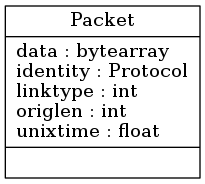
\includegraphics[scale=0.7]{diagrams/packet.png}
\caption{The packet class}
\end{figure}

Here, \emph{linktype} is an integer constant that represents one of many network media types. An important design decision was to make as few assumptions as possible about program input, so this field exists to identify what kind of packet this is. The most common value for this will be $1$, which corresponds to Ethernet (\texttt{LinkType.ETHERNET}) but other values are possible and should be supported.

The \emph{identity} is a field holds the root protocol (i.e. the bottom most protocol) instance for this packet. This is set to None by default, signifying the packet either has not been identified or has no known interpretation. More on this in the \emph{Protocols} section (\ref{sec:desproto}).

\subsection{Packet Sources}
\emph{Packet sources} are objects that support Python's \emph{iterator protocol} that yield the packet objects mentioned above. Packet sources are presented by the library as building blocks for higher level applications.
Packet sources represent a kind of lazily-evaluated interface towards streams of packets - this cuts down on memory usage, improving scalability. Sources that depend on other sources can be chained without restriction.

\subsection{Protocols}
\label{sec:desproto}
Network protocols are represented by Protocol classes. Protocol classes are the most complex abstraction.

Logically speaking, instances of communication over a network have a linear hierarchy of protocols. A \emph{carrier protocol} encapsulates another protocol, which itself may be another carrier protocol.

A carrier protocol will also have some kind of \emph{route}, a known source and destination. This may or may not depend  on the parent protocol. For instance, IP packets will typically be sent over Ethernet frames, but IP implements a logically independent network from an Ethernet network - these frames, when reaching a router, will be sent somewhere else (with altered frame data), potentially to entirely different routers over an entirely different carrier, all while preserving the IP frame. This is how internetworking works. Conversely, UDP packets rely on the logical route established by IP packets to transmit data, and are basically an extension of the \emph{protocol} or \emph{next} field in an IP header.

\begin{figure}[H]
\center
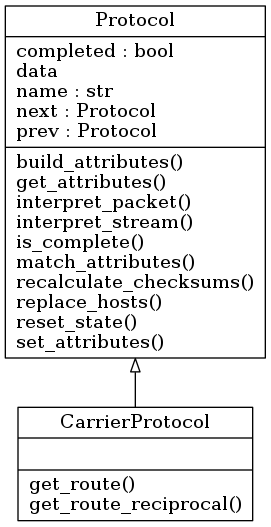
\includegraphics[scale=0.7]{diagrams/protocol.png}
\caption{The protocol and carrier protocol classes}
\end{figure}

The diagram above shows the design of the Protocol and CarrierProtocol classes. For any protocol to be represented in the program, it must have a Protocol class. This class has a well defined form, and this is important as extensibility 

Protocol classes have a single \emph{class variable} and three \emph{unbound methods} (static methods), in addition to the per-instance fields and bound methods typical of most classes. These are used to identify the protocol, and construct protocol instances respectively. A more detailed description of these is given below.

Firstly, every protocol instance has a field called data. This is intended to be used as a quasi-internal field, holding either a Python `memoryview' object or a `memorymap' object (see \ref{sec:memmap}). Python \texttt{memoryview} objects are effectively pointers to regions of memory held by objects supporting the \emph{buffer} protocol. A \texttt{memoryview} of a \texttt{bytearray} provides a read-write view of that data without requiring a direct reference to it. Like most python collections, \texttt{memoryview} objects support being sliced - this is important.

Because packets have a linear hierarchy of protocols, Protocol instances have a structure not unlike a linked list - each instance has a parent protocol (called \texttt{prev}) and a child protocol (called \texttt{next}); these are set to none if this is the bottom most or top most protocol, respectively.

Additionally, there is a boolean value called \texttt{completed}, which is to signify whether this protocol instance has finished being dissected. Setting this value to false allows other parts of the code to know that a packet has had its identification deferred until more information is available.

As for bound methods, there are 6 defined, \texttt{get_attributes}, \texttt{set_attributes}, \texttt{match_attributes}, \texttt{is_complete}, \texttt{recalculate_checksums} and \texttt{replace_hosts}.

The \texttt{is_complete}, \texttt{recalculate_checksums} and \texttt{replace_hosts} methods are all propagating methods - they will call their own equivalent on the child protocol instance, if any. \texttt{is_complete} works on the aformentioned \texttt{completed} boolean, returning true if and only if this value is true for all child protocols.

As replacing host identity information is one of the goals of the project, a \texttt{replace_hosts} method was defined. This takes a single argument, a dictionary. This dictionary defines a mapping between host identifiers and their replacements, the idea being that implementations of this method will look for possible substitutions and alter their instance data accordingly, and then call \texttt{replace_hosts} on the child instance. This provides a very simple and reliable way of doing this substitution. In a similar vein, \texttt{recalculate_checksums} is for updating any checksum data. Actual recalculation should start from the top most protocol instance, as the lower level carriers may have checksums on their payload (i.e. UDP).

The \texttt{get_attributes}, \texttt{set_attributes}, \texttt{match_attributes} (and \texttt{build_attributes})  methods all work with or produce  a set of \emph{protocol attributes}. The precise format of said attributes is entirely up to the implementing class, but is suggested to be a \emph{dictionary}.

\texttt{get_attributes} is supposed to return `attributes' of that protocol instance (for example, IPv4 attributes might contain the source/destination address and the protocol number). Conversely, \texttt{set_attributes} is supposed to alter packet data such that the packet corresponds to the attributes provided. \texttt{match_attributes} compares a set of attributes to those of the protocol instance - if they match, this method returns true, else false.

Protocol classes are also required to have a few unbound methods. The most important one, is \texttt{interpret_packet}. 
This method takes two arguments, a \texttt{memoryview} or \texttt{memorymap} object, and a \emph{parent} protocol instance. It is the job of this method to construct and return a protocol instance, possibly calling \texttt{interpret_packet} a subset of the data provided. This method is also responsible for maintaining state for completing deferred identification. \texttt{interpret_stream} effectively does the same thing, but for \emph{streams}.
Because both of these methods may have side effects, as a library, it was deemed appropriate to have some kind of mechanism for restoring the default set of state for these classes - this is the job of the \texttt{reset_state} method.

\texttt{build_attributes} is the last unbound method. This method is supposed to return attributes not unlike those returned by \texttt{get_attributes}, and is used for turning human input (an `attribute string') into a workable object.

Finally, all protocol classes need to have a human-readable name. This is for both output (such as when `printing' a packet) but mainly as a unique identifier for a Protocol class. The intention is, that protocols are referred to by this name, and that a Protocol class can be replaced by one with the same name, should the user want to use an alternate implementation. This name is also used in constructing and comparing attributes.

\section{Memory maps}
\label{sec:memmap}
In order to identify protocols, packet data needs to be examined. As some protocols can have a variety of carriers, and carrier protocols can have a variable size, the exact location of one protocol's header is not a constant offset.

The initial approach to this problem was just to copy the payload section of a protocol and present that to the next protocol interpreter. This works, but means any modifications would require the packet to be rebuilt - a time consuming operation.

Python \emph{memoryview} objects provide a memory-efficient and simple way of presenting smaller sections of data from an object. They are probably best illustrated with an example:
\begin{lstlisting}[
	language={[3]Python},
   	caption={[Memoryview demonstration]A demonstration of memoryviews. v is a view of data, and v1/v2 are subviews of data.}
]
>>> data = bytearray(b"abcdef")
>>> v = memoryview(data)
>>> bytes(v)
b'abcdef'
>>> v1 = v[0:3]
>>> v2 = v[3:6]
>>> bytes(v1)
b'abc'
>>> bytes(v2)
b'def'
>>> v2[1] = b"E"
>>> bytes(v)
b'abcdEf'
\end{lstlisting}
Here, some data object (called \texttt{data}) is being read and altered by some \emph{memoryview} objects (called \texttt{v}, \texttt{v1} and \texttt{v2}).

Importantly for this project, alterations to \emph{memoryview} objects affect their backing store - changes are reflected in the object the views are based on. These are sufficient to provide a linear tree of protocol instances with read/write access to packet data, but it was known from the start of the project that sometimes, parts of protocol data will exist over many packets.

For identification purposes, this can easily be solved by simply copying parts of the fragmented data and concatenating them. This solution is a different application of the first solution presented and suffers from all its downsides in addition to the problem of making alteration a very difficult task.

To solve this problem efficiently, a \emph{memorymap} class is needed. This class would provide logically contiguous access to multiple, separate \emph{memoryview} objects.

The ideal implementation would have a similar interface to that of \emph{memoryview} objects, and function as a drop-in replacement. This means protocol classes need not worry over how many packets their data is spread.

\chapter{Implementation}
Implementation started concurrently with design. Challenges encountered during implementation would change the design, and vice versa.

\section{Meta-Implementation}
While this section is not really about any specific implementation detail, it does cover noteworthy discipline used by the author \emph{while implementing}.

\subsection{Coding Style}
Some of the functional requirements (namely \ref{nfr:10} code structure and \ref{nfr:11} code documentation) effectively require code to be well-written and well-documented.

To this end, a variant of the standard Python code style was used. In essence:
\begin{enumerate}[label=\roman*)]
\item Indentation is done with four spaces.\\
\item \emph{Private} fields in a class start with an underscore.\\
\item Functions and methods are lower\textunderscore{}case\textunderscore{}with\textunderscore{}underscores.\\
\item Constants are CAPITALS\textunderscore{}WITH\textunderscore{}UNDERSCORES.\\
\item Class identifieirs are written in UpperCamelCase.
\end{enumerate}
\subsection{Version Control}

\pagebreak
\section{The \texttt{memorymap} Module}
The \texttt{memorymap} module implements the \emph{memorymap} class as described in \ref{sec:memmap}, and works by mapping multiple \emph{memoryview} objects to a single \emph{logical} `index space'.

The \texttt{memorymap} class stores each constituent \emph{memoryview} object (denoted $V$) as part of a three-tuple,  with their \emph{logical} starting and ending index ($min$ and $max$, respectively). This tuple is henceforth referred to as a \emph{segment} (or $S$). These segments are stored in a list ($Q$), in ascending order of ranges.

{\small
A note on notation: Slightly non-standard notation and concepts have been employed to make this mathematical model more readable and understandable. \emph{Lists} are \emph{tuples} with different notation.

For a tuple, superscript denotes a component, i.e.  for tuple $T = (a,\, b,\, c\, ...)$,   $T^{a} = a$.

For a list, square brackets denote a specific element, i.e. for list $R = (\pi,\, \epsilon,\, \lambda\, ...)$, $R[3] = \lambda$
}

\begin{align*}
S_{i} &= ( V_{i},\, min_{i},\, max_{i} )\\
Q &= [ S_{0},\, S_{1},\, S_{2}\, ... \,S_{i} ]\\
\end{align*}
\begin{center}
Given $S_{a}$ and $S_{b}$ as any two elements in $Q$, where $a < b$,
\end{center}
\begin{align*}
&\ S_{a}^{max} \leq S_{b}^{min} 
\end{align*}

A \emph{logical index} ($n_{logical}$) is translated to a pair of actual indices, the \emph{segment index} ($n_{segment}$), which refers to one of the segments in the segment list, and a \emph{local index} ($n_{local}$), which is the part of the segment.

This translation is done by a very simple algorithm. A binary search of the segment list is done, identifying the range encompassing a \emph{logical index}.

\begin{align*}
n_{segment} &= search(Q,\,n_{logical})\\
N &= Q[n_{segment}]\\
n_{local} &= n_{logical} - N^{min}
\end{align*}

\section{The \texttt{common} Module}
\section{The \texttt{capfile} Package}
\section{The \texttt{identity} Package}
\subsection{Protocol classes}
In the default implementation of \texttt{match_attributes}, \texttt{get_attributes} is called.

The default implementation of \texttt{match_attributes}
\section{The \texttt{pipeline} Package}

\chapter{Testing}

\section{Testing approaches}

\section{Testing During Development}
\subsection{Regression Testing}

\chapter{Critical Evaluation}

\section{Successes}

\section{Failures}

\section{Retrospective Design Criticisms}

\section{Retrospective Method Criticisms}


\chapter{Appendix}
\section{Formats}
Pcap file format.


%%%%%%%%%%%%%%%%
% Bibliography %
%%%%%%%%%%%%%%%%

\begin{thebibliography}{99}
\bibitem{editcap-man}
    Richard Sharpe, Guy Harris, Ulf Lamping (4th of March, 2015)\\
    EDITCAP (1), The Wireshark Network Analyzer

\bibitem{tshark-man}
    Gerald Combs, numerous others (4th of March, 2015)\\
    WIRESHARK (1), The Wireshark Network Analyzer

\bibitem{tcpreplay-web}
    Aaron Turner, Fred Klassen\\
    tcpeplay home page(s).
    \url{http://tcpreplay.appneta.com}\\
    (see also: \url{http://tcpreplay.synfin.net/})

\bibitem{bittwist-web}
    Addy Yeow Chin Heng\\
    libpcap-based Ethernet packet generator.\\
    \url{http://bittwist.sourceforge.net/}

\bibitem{tcpl}
	Brian W. Kernighan, Dennis M. Ritchie (1988)\\
	The C Programming Language, 2nd edition.

\bibitem{tcpppl}
	Bjarne Stroustrup (1997)\\
	The C++ Programming Language, 3rd edition.

\bibitem{gcj}
	The GCC Team (30th of June, 2014)\\
	The GNU Compiler for the Java Programming Language\\
	\url{https://gcc.gnu.org/java/}

\bibitem{javatech}
	Oracle Corporation (Accessed April, 2015)\\
	`Learn about Java Technology'\\
	\url{https://www.java.com/en/about/}

\bibitem{haskfunc}
    Simon Peyton Jones (December, 2014)\\
    The Haskell 98 Report\\
    \url{https://www.haskell.org/onlinereport/intro.html}

\bibitem{mono}
	Mono Project (Accessed April, 2015)\\
	Cross platform, open source .NET framework\\
	\url{http://www.mono-project.com}

\bibitem{cpy2maint}
    Various authors (13th of April, 2014)\\
    Should I use Python 2 or Python 3 for my development activity?\\
    \url{https://wiki.python.org/moin/Python2orPython3}

\bibitem{qcou}
    Peter H. Salus. (1st of June, 1994)\\
    A Quarter-Century of Unix

\bibitem{wwr-waterfall-notes}
    Dr. Winston W. Royce (26th August, 1970)\\
    MANAGING THE DEVELOPMENT OF LARGE SOFTWARE SYSTEMS\\
    \url{http://www.cs.umd.edu/class/spring2003/cmsc838p/Process/waterfall.pdf}
    
\bibitem{ieee802.3}
	IEEE Computer Society (28th December, 2012)
	IEEE Standard for Ethernet (IEEE Std 802.3-2012)
	\url{http://standards.ieee.org/getieee802/download/802.3-2012_section1.pdf}
	
\bibitem{rfc826}
	David C. Plummer (November, 1982)\\
	An Ethernet Address Resolution Protocol, or\\
	Converting Network Protocol Addresses\\
	\url{https://tools.ietf.org/html/rfc826}
	
\bibitem{rfc791}
	Information Sciences Institute, University of Southern California (September, 1981)\\
	INTERNET PROTOCOL\\
	\url{https://tools.ietf.org/html/rfc791}
	
\bibitem{rfc2460}
	S. Deering, R. Hinden, The Internet Society (December 1998)\\
	Internet Protocol, Version 6 (IPv6)\\
	\url{https://tools.ietf.org/html/rfc2460}

\end{thebibliography}
\end{document}
